%Focus generale sulle tecnologie utilizzate
In this section, we outline the technical aspects concerning the realization of our solution. Therefore, we first present the enabler technologies through which we instantiate the architectural principles presented in \cref{sec:design}. After that, we discuss the CONFINE interaction protocol. Finally, we show the implementation details.

%
\begin{figure}[t]
	\centering
	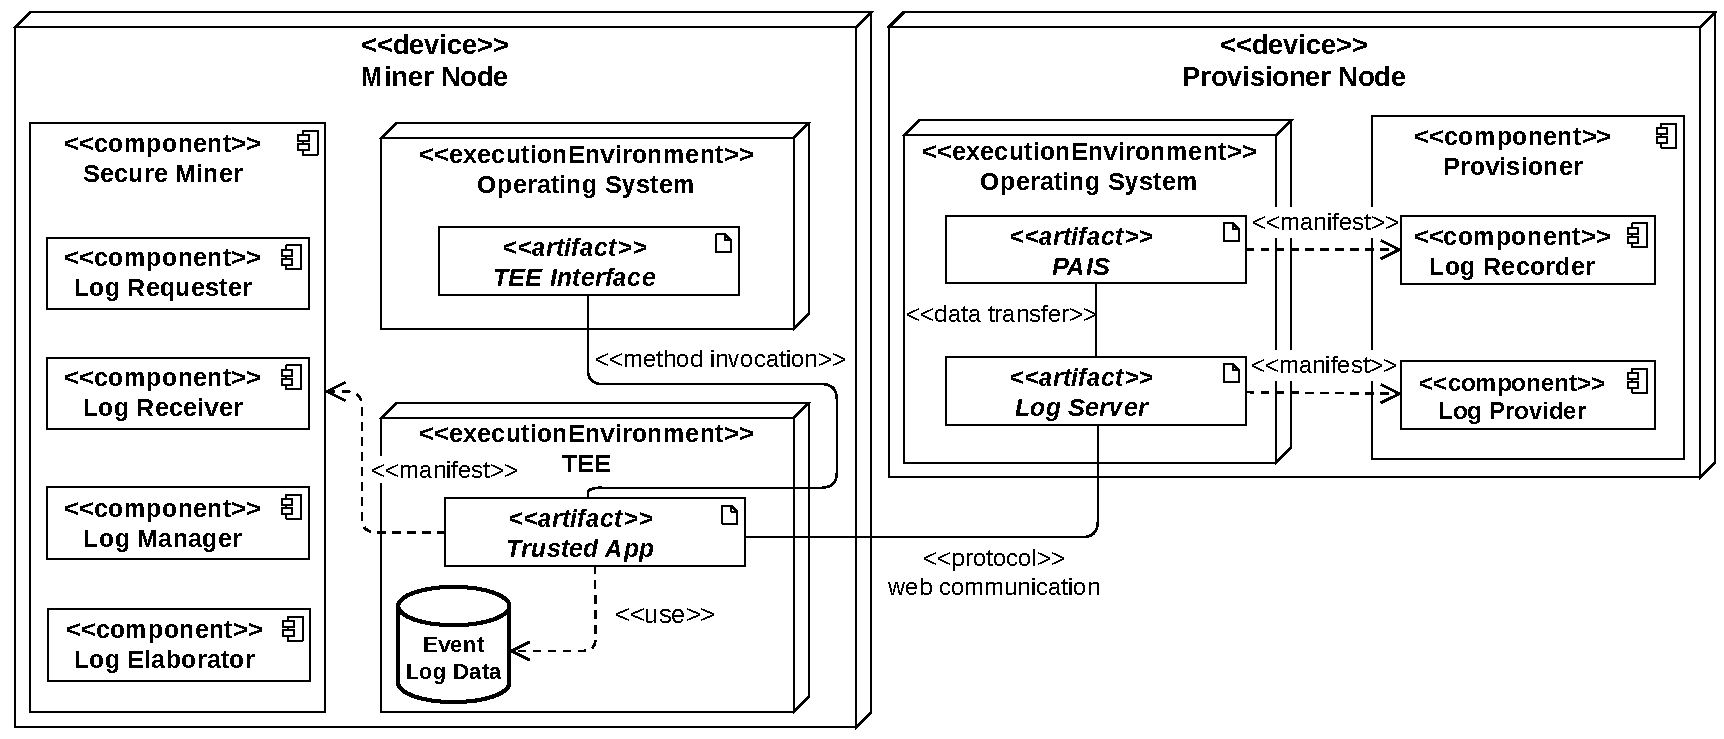
\includegraphics[width=1\linewidth]{content/figures/deploymentdiagram.pdf}
	\caption{UML deployment diagram of the CONFINE architecture}
	\label{fig:deployment_diagram}
\end{figure}
%
\subsection{Deployment}
\label{sec:deployment}
%
%As follows, we bridge the gap between the CONFINE high-level architecture and its practical realization. 
\Cref{fig:deployment_diagram} depicts a UML deployment diagram~\citep{koch2002expressive} to illustrate the employed technologies and computation environments. %that aims to help with understanding the instantiated technologies. We differentiate between the technologies designated for mining, denoted as \Compo{Miner Node}s, and those specifically associated with provisioners, identified as \Compo{Provisioner Node}s. To enhance clarity, we maintain the separation of these \textit{devices} in the accompanying diagram. However, organizations have the flexibility to opt for integrated technologies that incorporate both mining and provisioning functionalities. 
We recall that the \Compo{Miner} and \Compo{Provisioner} nodes are drawn as separated, although organizations can host both.
In our motivating scenario, e.g., the \Actor{Hospital} can be equipped with machines aimed for both mining and provisioning. %, while the \Actor{Specialized clinic} can make use of separate devices. 
% We included the \texttt{Log Recorder}, the \texttt{Log Provider}, and \texttt{Secure Miner} (already discussed in \cref{sec:design}) as abstract \textit{components} of the diagram, whose manifestations are described as follows. 

\Compo{Provisioner Node}s host the \Compo{Provisioner}'s components, encompassing the \Compo{Log Recorder} and the \Compo{Log Provider}. 
The Process-Aware Information System (\Compo{PAIS}) manifests the \Compo{Log Recorder}~\citep{Dumas.etal/2018:FundamentalsofBPM}. % which plays a crucial role in managing various business processes, including accounting and resource management . In our motivating scenario, the \Actor{Hospital} and the other provisioners record Alice and Bob's cases through this class of systems.
%
%
The \Compo{PAIS} grants access to the \Compo{Log Server}, enabling it to retrieve event log data. The \Compo{Log Server}, on the other hand, embodies the functionalities of the \Compo{Log Provider}, implementing web services aimed at handling remote data requests and providing event log data to miners. %The \Actor{Hospital}, the \Actor{Specialized Clinic}, and the \Actor{Pharmaceutical Company} of our running example employes \Compo{Log Servers} adhering to established web standards such as HTTP\footnote{\url{w3.org/Protocols/rfc2616/rfc2616.html}. Accessed: \today.}, FTP\footnote{\url{w3.org/Protocols/rfc959/}. Accessed: \today.}, and Goopher\footnote{\url{datatracker.ietf.org/doc/html/rfc1436}. Accessed: \today.}. 
% ^The \Compo{PAIS} and \Compo{Log Server} run on the top of the \Compo{Operating System} of the \Compo{Provisioner Node}.

The \Compo{Miner Node} is characterized by two distinct \textit{execution environments}: the \Compo{Operating System} (\Compo{OS}) and the Trusted Execution Environment (\Compo{TEE})~\citep{DBLP:conf/trustcom/SabtAB15}. \Compo{TEE}s establish isolated contexts separate from the \Compo{OS}, safeguarding code and data through hardware-based encryption mechanisms. This technology relies on %specialized %components of the \Compo{Miner Node}'s 
dedicated sections of a CPU capable of handling encrypted data within a reserved section of the main memory~\citep{costan2016intel}.
By enforcing memory access restrictions, TEEs aim to prevent one application from reading or altering the memory space of another, thus enhancing the overall security of the system.
These dedicated areas in memory are, however, limited.
Once the limits are exceeded, TEEs have to scout around in outer memory areas, thus conceding the opportunity for malicious readers to understand the saved data based on the memory reads and writes.
To avoid this risk, TEE implementations often raise errors that halt the program execution when the memory demand goes beyond the available space. %dedicated to a trusted application is exceeded. %, are generated and execution is halted.
Therefore, the design of secure systems that resort to TEEs must take into account that memory consumption must be kept under control.
%TEEs incorporate defined memory constraints as a deliberate measure to augment security and establish a secure demarcation for sensitive computational processes. 
We leverage the security guarantees provided by \Compo{TEE}s~\citep{DBLP:journals/ieeesp/JauernigSS20} to protect a \Compo{Trusted App} responsible for fulfilling the functions of the \Compo{Secure Miner} and its associated sub-components. %The \Compo{Trusted App} consolidates the logic required for generating verifiable data requests, receiving external event logs, securely storing them within the \Compo{TEE}, and executing process mining algorithms. %All procedures executed by the \Compo{Trusted App} are tamper-proof. 
The \Compo{TEE} ensures the integrity of the \Compo{Trusted App} code, protecting it against potential malicious manipulations and unauthorized access by programs running within the \Compo{Operating System}. Additionally, we utilize the isolated environment of \Compo{TEE}s to securely store event log data (e.g., Alice and Bob's cases).
\begin{newj}
{The \Compo{Trusted App} can be identified as a \Compo{Secure Miner} application through its \emph{measurement}, which is defined as the hash value of the combination of its source code and data at the deployment stage.} 
\end{newj}
% from provisioner organizations within the \Compo{Miner Node}. 
\begin{newj}
% The \Compo{TEE} retains a private key in the externally inaccessible section of memory  paired with a public key in a Rivest-Shamir-Adleman\todo{The coprocessor’s attestation key is stored in battery-backed memory that is only accessible to the service processor} (RSA)~\citep{DBLP:journals/cacm/RivestSA83} scheme for attestation (only the owner of the private key can sign messages that are verifiable via the public key) and secure message encryption (only the owner of the private key can decode messages that are encrypted with the corresponding public key). The private key associated with the \Compo{TEE}'s hardware remains inaccessible, even to users possessing administrative privileges on the \Compo{Miner Node}
%, preventing exposure to the \Compo{Operating System}.
The \Compo{TEE} retains an \Compo{Attestation Key} in the externally inaccessible section of memory paired with a public key owned by the CPU manufacturer. The \Compo{Attestation Key} is permanently burned into the CPU fuses, ensuring its accessibility solely to the hardware when attesting the \Compo{Trusted App} nature for \Compo{Provisioner}s. We provide further details concerning the attestation mechanism in the following subsection.  %The private key associated with the \Compo{TEE}'s hardware remains inaccessible, even to users possessing administrative privileges on the \Compo{Miner Node}.
\end{newj}
In our solution, access to event log data located in the \Compo{TEE} is restricted solely to the \Compo{Trusted App}. Users interact with the \Compo{Trusted App} through the \Compo{Trusted App Interface}, which serves as the exclusive communication channel. The \Compo{Trusted App} offers secure methods, invoked by the \Compo{Trusted App Interface}, for safely receiving information from the \Compo{Operating System} and outsourcing the results of computations. %, maintaining a high level of data security.

\begin{comment}
\begin{figure}[t]
\centering
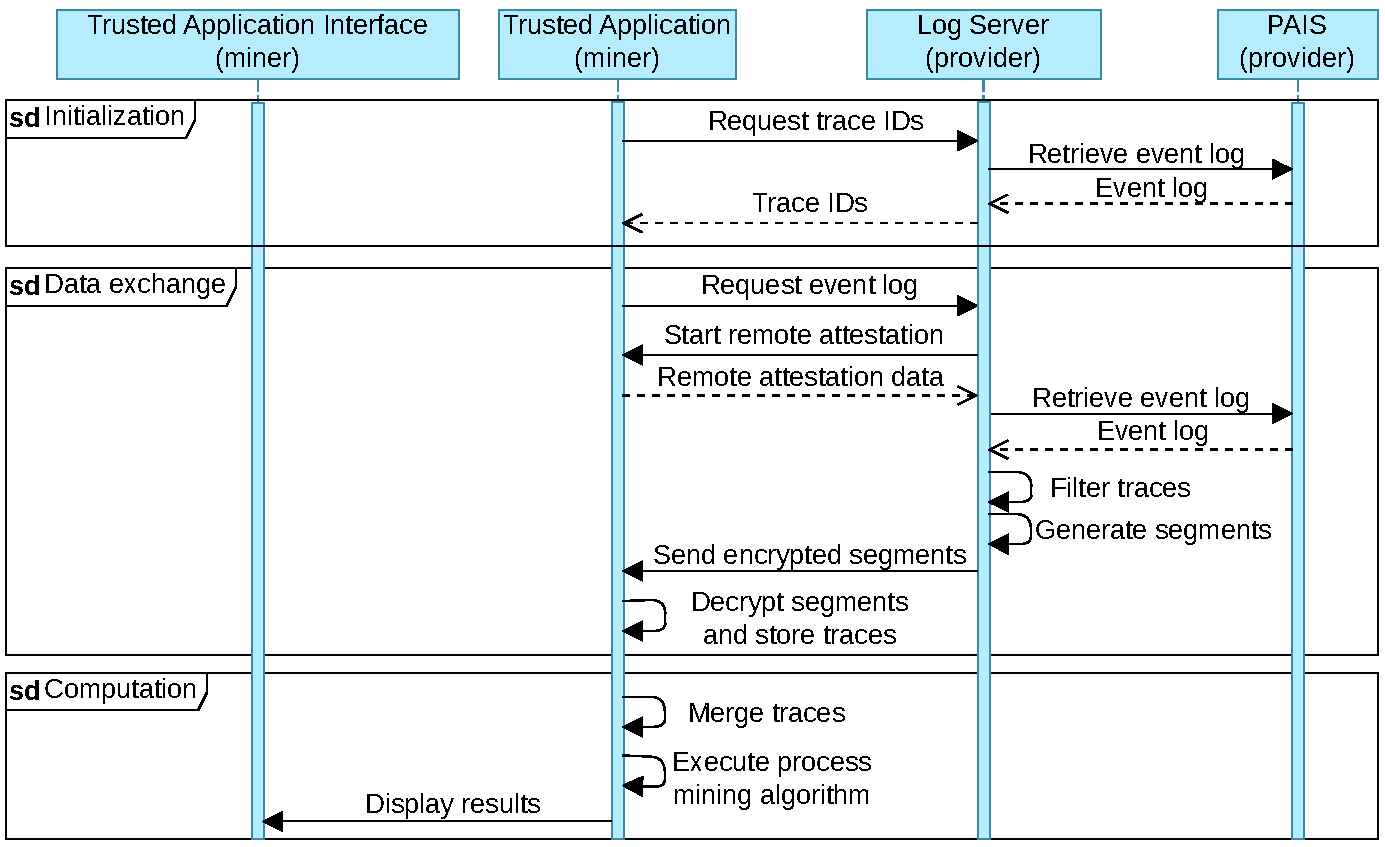
\includegraphics[width=0.9\linewidth]{content/figures/sequencediagram.pdf}
\caption{UML sequence diagram.}
\label{fig:sequence_diagram}
\end{figure}
\end{comment}


\subsection{The CONFINE protocol}
\label{sec:deployment:protocol}
We orchestrate the interaction of the components in CONFINE via a protocol. We separate it in four subsequent stages, namely
\begin{inparaenum}[\itshape(i)\upshape]
	\item \textit{initialization}, \item \textit{remote attestation}, \item \textit{data transmission}, and \item \textit{computation}.
\end{inparaenum}
These stages are depicted in \cref{fig:init,fig:attestation,fig:transmission,fig:computation}, respectively.
\begin{comment}
\todo[inline]{Assumptions.
``We assume that every process executes the code triggered by events in a mutually
exclusive way. This means that the same process does not handle two events concur-
rently. Once the handling of an event is terminated, the process keeps on checking
if any other event is triggered. This periodic checking is assumed to be fair, and is
achieved in an implicit way: it is not visible in the pseudo code we describe.''~\citep{Cachin.etal/2011:ReliableSecureDistributedProgramming}
``(Regular) reliable brodcast, (d’ora in poi solo Reliable broadcast) :
Safety. 
Integrity (No Duplication, No Creation): per qualsiasi messaggio m, ogni processo corretto consegna m al più una volta, e solo se m è stato precedentemente inviato in broadcast da un processo mittente
Liveness:
Validity: se un processo corretto invia in broadcast un messaggio m, allora tutti i processi corretti alla fine consegnano m.
Agreement : se un processo corretto consegna un messaggio m, allora tutti i processi corretti alla fine consegnano m.''
I provisioner e il miner devono essere corretti, i.e., they do not crash.~\citep{Cachin.etal/2011:ReliableSecureDistributedProgramming}
\\
We resort to the following:
``a general-purpose secure transport
layer protocol, such as SSL/TLS~\citep{Thomas/2000:SSL-TLS}. The secure transport protocol provides a
secure channel to the application layer, i.e., it provides a communication channel
with some extra security services; for example, the secure channel may prevent
an attacker from faking messages, hijacking messages (redirecting them to an
unintended recipient, or reascribing them so that they seem to have come from
a different sender), or learning the content of messages.''~\citep{KamilLowe/FAST2010:AbstractionsSecureChannels} 
}
\end{comment}
Our protocol involves two primary entities: a \Compo{Secure Miner} (hereafter referred to as \SecM) and one or more \Compo{Provisioner}s ($\LPrv_1, \ldots, \LPrv_n \in \LPrvS$). 
\begin{newj}
The behavioral descriptions for {\SecM} and any $\LPrv_i \in \LPrvS$  are outlined in \cref{alg:secm} and \cref{alg:lprv}, respectively. These specifications adhere to the syntax for distributed algorithms detailed in \cite{Cachin.etal/2011:ReliableSecureDistributedProgramming}.% 
\footnote{In order to enhance clarity, we adapt the original syntax of the \Mesg{Deliver} and \Mesg{Send} expressions to emphasize message senders (preceded by the symbol `$\ll$') and receivers (preceded by `$\gg$') respectively.}
We assume that communication between \Compo{Secure Miner}s and \Compo{Log Provisioner}s occurs through an \textit{Authenticated Point-to-Point Perfect Link} \cite{Cachin.etal/2011:ReliableSecureDistributedProgramming}. This communication abstraction guarantees:
\begin{inparaenum}[\itshape(i)\upshape]
\item \textit{reliable delivery} (i.e., if a correct process sends a message \textit{m} to a correct
process \textit{q}, then \textit{q} eventually delivers \textit{m}),
\item \textit{no duplication} (i.e., no message is delivered by a correct process more than once), and
\item \textit{authenticity} (i.e., if some correct process \textit{q} delivers a message \textit{m} with sender \textit{p}
and process \textit{p} is correct, then \textit{m} was previously sent to \textit{q} by \textit{p}). 
\end{inparaenum} We posit the assumption that communications transmitted throughout protocol execution are safeguarded by end-to-end encryption. Therefore, the content of the messages is discernible solely to the designated sender and receiver.

In \cref{alg:secm}, the \Compo{Secure Miner} is provided with the following input:
\begin{inparadesc}
    \item the list of \Compo{Provisioner}s' references ($\LPrv_1, \ldots, \LPrv_n$), namely descriptors all the necessary information to locate and identify provisioners, and 
    \item a segment size {\SegSize} employed for the log segmentation during the \textit{data transmission} phase.\todo[inline]{Controlla che la seg size e la segmentazione sono state introdotte. la seg size ha come dimensione minima la grandezza della traccia piu grande nel log, come dimensione massima la portata della TEE. Assumiamo che la somma dei pezzi di traccie sia piu grande della dimensione massima consentita diviso il numero di} 
\end{inparadesc}
Similarly, the \Compo{Provisioner}'s specification in \cref{alg:lprv} considers as input the list of references to miners ($\SecM_1, \ldots, \SecM_s$) for which event log access is enabled. According to the underlying syntax, {\SecM} and {\LPrv} execute code prompted by events mutually exclusively, implying that they do not concurrently manage two events. For the sake of clarity, we omit any explicit representation of this feature in the pseudo-codes under discussion.
\end{newj}

In the following, we describe each protocol phase in detail.

\begin{figure}[t]
	\subfloat[][Initialization]{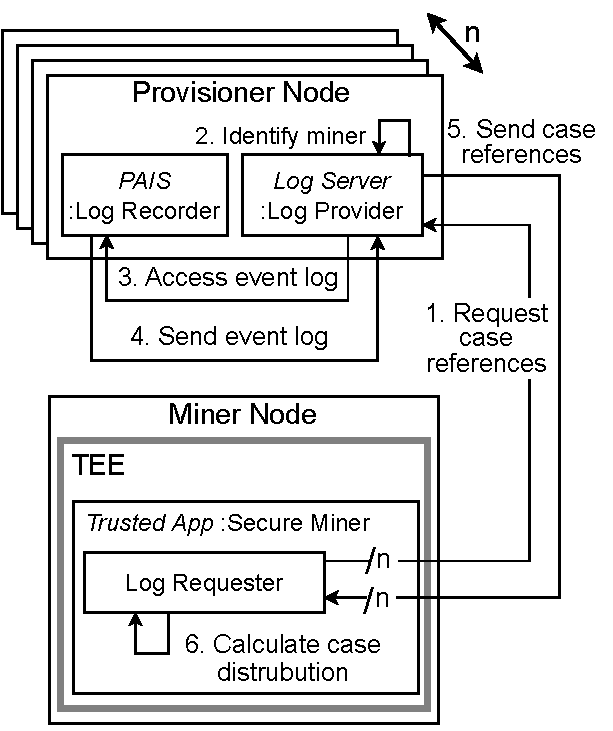
\includegraphics[width=0.45\linewidth]{content/figures/initializationworkflow.pdf}\label{fig:init}}\hfill
	\subfloat[][Remote attestation]{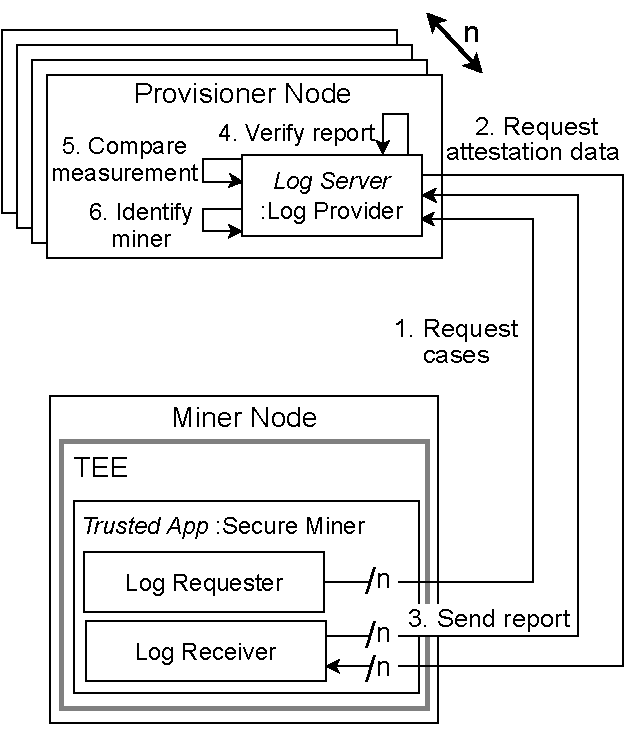
\includegraphics[width=0.45\linewidth]{content/figures/attestationworkflow.pdf}\label{fig:attestation}}\hfill
	\caption{Unfolding example for the initialization and remote attestation phases of the CONFINE protocol}
	\label{fig:workflow}
\end{figure}

\noindent\textbf{Initialization.} The objective of the initialization stage is to inform the miner about the distribution of cases related to a business process among the \Compo{Provisioner Node}s. At the onset of this stage, the \Compo{Log Requester} within the \Compo{Trusted App} issues $n$ requests, one per \Compo{Log Server} component, %of the provisioners 
to retrieve the list of case references they record (step 1 in \cref{fig:init} and \crefalgln[alg:secm]{alg:secm:CaseRefsReq:call}). Following sender authentication (2), each \Compo{Log Server} retrieves the local event log from the \Compo{PAIS} (3, 4) and subsequently responds to the \Compo{Log Requester} by providing a list of its associated case references (5 and \crefalgln[alg:lprv]{alg:lprv:sendRefs}). After collecting these $n$ responses (\crefalgln[alg:secm]{alg:secm:respcollection}), the \Compo{Log Requester} delineates the distribution of cases. In the context of our motivating scenario, by the conclusion of the initialization, the miner gains knowledge that the case associated with Bob, synthesized in the traces $T^H_{711}$ and $T^C_{711}$, is exclusively retained by the \Actor{Hospital} and the \Actor{Specialized Clinic}. In contrast, the traces of Alice's case, denoted as $T^H_{312}$, $T^C_{312}$, and $T^S_{312}$, are scattered across all three organizations.

%\begin{comment}
\begin{algorithm2e}[tb]
	% !TeX encoding = utf8
% !TeX root = ../main.tex
%
\begin{comment}
	% See macros file
	\def\LPrv {\ensuremath{\mathcal{P}}}   % Log provider
	\def\SecM {\ensuremath{\mathcal{M}}}   % Secure Miner
	\def\LPrvS {\ensuremath{\widehat{\mathcal{P}}}}  % Log provider set
	\def\CStor {\ensuremath{\textrm{Cases}}}  % Case store 
	\def\Case {\ensuremath{c}}  % Case 
	\def\CasP {\ensuremath{\textrm{casePart}}}  % Case part
	\def\CId {\ensuremath{\textrm{cid}}}  % CaseId
	\def\CIdU {\ensuremath{\widehat{\textrm{CID}}}}  % CaseId universe
	\def\CS {\ensuremath{C}}  % Case set
	\def\CasU {\ensuremath{\widehat{C}}}  % Case universe
	\def\CIdS {\ensuremath{\textrm{CIDs}}}  % CaseId set
	\def\CIDMap {\ensuremath{\textrm{CIDMap}}} % CaseId Map
	\def\LPrvMap {\ensuremath{\textrm{PMap}}} % Log provider Map
	\newcommand{\Mesg}[1]{\ensuremath{\textrm{\textsc{#1}}}}
	\newcommand{\SuchThat}[1]{~\upshape\textrm{\textbf{such that}}~{#1}}
	\newcommand{\To}[1]{~\upshape\textrm{\textbf{to}}~{#1}}
	\newcommand{\Call}[1]{\texttt{#1}}
	
	\def\SegSize {\ensuremath{\textrm{seg\_size}}}
	\def\Segm {\ensuremath{S}}
\end{comment}

\tiny
% \scriptsize
\DontPrintSemicolon \SetAlgoVlined \SetInd{0.3em}{1em}
\setstretch{1.1}

\KwIn{%
	$\LPrvS = \{ \LPrv_1, \ldots, \LPrv_n \}$, the (references to) $n$ log provisioners;%
	\newline
	$\SegSize$, the maximum size of the log segment to be transmitted by the log provisioners;%
	%	\newline%
	%	$\DecRepertoire$, a finite set of {\Declare} templates to be considered to express the discovered specification;%
	%	\newline%
	%	$\ProActvts \subseteq \Uact$, a finite set of activities to be included in the discovered specification;%
	%	\newline%
	%	$\MinThrld{\ConfTr}$, $\MinThrld{\SuppTr}$, $\MinThrld{\ConfEv}$, $\MinThrld{\SuppEv}$, the minimum thresholds for trace-based confidence and support, and event-based confidence and support, respectively (default for all four paramenters: $0.0$); %the minimum support 
}
\KwData{%
	$\CIDMap : \CIdU \to 2^{\LPrvS}$, a map from case references $\CId \in \CIdU$ to the set of log provisioners in $\LPrvS$ ; \newline%
	$\LPrvMap : \LPrvS \to 2^{\CIdU}$, a map from log provisioners $\LPrv \in \LPrvS$ to the set of references to their cases in $\CIdU$ ; \newline%
	$\CStor : \CIdU \to \CasU$, a map from case references $\CId \in \CIdU$ to a set of cases in $\CasU$
}
%\KwOut{%
	%	$\DecSpec$, a declarative process specification
	%}
\Implements{\Compo{SecureMiner} \SecM}
\Uses{\Compo{LogProvisioner} \LPrv}

\begin{comment}
	\todo{For an extended version, we should enlarge this pseudocode with the full interface}
	\Fn{\Call{getAttestationReport}(\LPrv) \SuchThat{$\LPrv \in \LPrvS$} \label{alg:getAttestationReport}}{
		\Return {attestation\_report}
	}
\end{comment}

\BlankLine
% 
%\ForEach{$\LPrv \in \LPrvS$ \tcc*[r]{For every log provider $\LPrv$}}{%
	%	$\CaseIdS \gets \CaseIdS \cup \LPrv.\CaseIdS$; \tcc*[r]{Register the $\LPrv$'s case reference list}%
	%	
	%}
\UponEv(\tcp*[f]{The \textit{initialization} phase begins here -- \cref{fig:init}}){\upshape $\langle \SecM.\Compo{LogRequester}, \Mesg{Init} \:|\: \LPrvS, \SegSize \rangle$}{
	\ForEach(\tcp*[f]{For every \Compo{Log Provider} $\LPrv$}){$\LPrv \in \LPrvS$}{%
		\Trigger{\upshape $\langle \LPrv.\Compo{LogProvider}, \Mesg{CaseRefsReq} \:|\: \SecM \rangle$\label{alg:CaseRefsReq:call}} \tcp*{Request its case references (see \hyperref[alg2:CasesRefReq]{Alg.2, Line \ref{alg2:CasesRefReq}})}
	}
	\Upon(\tcp*[f]{Once all $\LPrv$s have answered with their case references}){\upshape $|\LPrvS| = |\textrm{dom}(\LPrvMap)|$}{%
		\lForEach%(\tcp*[f]{For every reference to the \Compo{Log Provider} $\LPrv'$})
		{$\LPrv \in \LPrvS$}{
			\Trigger{\upshape $\langle \LPrv.\Compo{LogProvider}, \Mesg{CasesReq} \:|\: \SecM, \SegSize, \LPrvMap[\LPrv] \rangle$\label{alg:CasesReq:call}}
			\tcp*[f]{Request their cases (see \hyperref[alg2:CasesReq]{Alg.2 Line \ref{alg2:CasesReq}})}
			%\tcc*{Request the cases that are provided by $\LPrv'$. Before sending them, $\LPrv'$ will trigger \Mesg{AttestReportReq} in return, to attest the \Compo{Secure Miner}.}
		}
	}
}
\UponEv(\tcp*[f]{{\SecM} gets the case references (see \hyperref[alg2:sendRefs]{Alg.2, Line \ref{alg2:sendRefs}})}){\upshape $\langle \SecM.\Compo{LogRequester}, \Mesg{CaseRefsRes} \:|\: \LPrv, \CIdS \rangle$ \SuchThat{$\LPrv \in \LPrvS$} \label{alg:CaseRefsRes}}{
	\ForEach(\tcp*[f]{For every case reference $\CId$}){\upshape $\CId \in \CIdS$}{%
		$\CIDMap[\CId] \gets \CIDMap[\CId] \cup \{\LPrv\} $ \tcp*{Add $\LPrv$ to the set of providers for case $\CId$ in $\CIDMap$}
	}
	$\LPrvMap[\LPrv] \gets \LPrvMap[\LPrv] \cup \CIdS $ \tcp*{Register the references of the cases provided by $\LPrv$ in $\LPrvMap$}
}

\UponEv(\tcp*[f]{$\SecM$ gets segments from {\LPrv} (see \hyperref[alg2:sendSegs]{Alg.2 line 9})}){\upshape $\langle \SecM.\Compo{LogReceiver}, \Mesg{CasesRes} \:|\: \LPrv, \Segm \rangle$ \SuchThat{$\LPrv \in \LPrvS$} \label{alg:CasesRes} }{
	% See {\LaTeX} comments\\
	% Per ogni pezzo-di-caso ricevuto nel segmento, controlla che il provider sia stato dichiarato in possesso di esso
	% SE PMap ha ancora il CID
	% Aggiungi il pezzo-di-caso alla lista di pezzi-di-caso associati a quell'id
	% Togli il CID del pezzo-di-caso da PMap in P
	% Togli il P dal CIDMap
	% upon CIDMap vuoto in un CID, mergia e yielda il caso
	\ForEach(\tcp*[f]{For every $\CasP_\CId$ in the delivered set of segments $\Segm$, each associated with a \CId}){\upshape $\CasP_\CId \in \Segm$}{%
		\If(\tcp*[f]{The store phase (see \cref{fig:transmission})}){\upshape $\CId \in \LPrvMap[\LPrv]$}  {%
			$\LPrvMap[\LPrv] \gets \LPrvMap[\LPrv] \,\setminus\, \{\CId\}$ \tcp*[f]{\raggedright Remove {\CId} from the set of cases to be provided by {\LPrv}}
			$\CIDMap[\CId] \gets \CIDMap[\CId] \,\setminus\, \{\LPrv\}$ \tcp*[f]{Remove $\LPrv$ from the set of $\CId$ providers}
			$\Compo{LogManager}.\Call{mergeAndStore}\left(\CStor, \CasP_\CId\right)$ \tcp*[f]{Update the case via $\Merge$ and store the result in {\CStor}}
		}
	}
}

\Upon(\tcp*[f]{When all the pieces of some $\CId$ have arrived} to \SecM){\upshape $\CIDMap[\CId]= \emptyset$ for some $\CId \in \textrm{dom}(\CIDMap)$} {%
	$\textrm{dom}(\CIDMap) \gets \textrm{dom}(\CIDMap) \,\setminus\, \{\CId\}$\tcp*[f]{Remove $\CId$ from the $\CId$ domain which still needs to be processed}\;
	\Yield{\upshape \CStor[\CId] \To{}} \Compo{LogElaborator} \tcp*[f]{forward the $\CId$ to the \Compo{Log Elaborator} for mining (\cref{fig:computation})}
}

\endinput
UPON EVENT(M,CASERES|P,S) SUCH THAT P in \widehat{\mathcal{P}} DO
	for each C ∈ S:
		if C.cid ∈ PMap[P]
			CMap[C.cid]<--CMap[C.cid] ∪ {C}
			PMap[P]<-- PMap[P] \ {C.cid}
			CIDMap[C.cid]<-- CIDMap[C.cid] \ {P}


UPON |CIDMap[cid]|=0 such that cid in dom(CIDMap) //Computation phase start here.
merge all traces in CIDMap[cid] using mergingSchema and put it in mergedTrace
yeld PMAlgorithm(mergedTrace)

	\caption{Secure Miner's behavior in CONFINE.}
	\label{alg:secm}
\end{algorithm2e} 
%\end{comment}
%\begin{comment}
\begin{algorithm2e}[tb]
	\tiny
% \scriptsize
\DontPrintSemicolon \SetAlgoVlined \SetInd{0.3em}{1em}
\setstretch{1.1}
% Additional macros in addon/macros.tex and addon/utils.tex

\KwIn{%
	$\SecMS = \{ \SecM_1, \ldots, \SecM_s \}$, the (references to) $s$ miners.%
}

\Implements{\Compo{Provisioner}, {\Inst} {\LPrv}.}
\Uses{\textit{AuthenticatedPerfectPointToPointLink}, {\Inst} {\AuthPtP}.}
\UponEv(\tcp*[f]{{\LPrv} receives the request for case references from {\SecM} (see \crefalgln[alg:secm]{alg:secm:CaseRefsReq:call})}){$\langle \AuthPtP, \Mesg{Deliver} \:|\: \SecM,[\Mesg{CasesRefsReq}] \rangle$ \label{alg:lprv:CasesRefReq}\SuchThat{$\SecM \in \SecMS$}}{%
	%\If(\tcp*[f]{Authenticate the sender miner {\SecM}}){\LPrv.\Compo{LogProvider}.\Call{authenticateMiner}(\SecM) is successful}{
            $\CIdS \gets \LPrv.{\Compo{LogRecorder}}.\Call{accessCaseReferences()}$\tcp*[f]{Access the case references via \Compo{Log Recorder}}\\
            \Trigger{$\langle \AuthPtP, \Mesg{Send} \:|\: \SecM,[\Mesg{CasesRefRes},\CIdS] \rangle$ } \tcp*[f]{{send the case references to {\SecM} (see \crefalgln[alg:secm]{alg:secm:CaseRefsRes})\label{alg:lprv:sendRefs}}}
	%}
}
\UponEv(\tcp*[f]{{\LPrv} gets the case request from {\SecM} (see \crefalgln[alg:secm]{alg:secm:CasesReq:call})}){$\langle \AuthPtP, \Mesg{Deliver} \:|\: \SecM, [\Mesg{CasesReq},\SegSize, \CIdS]\rangle$ \label{alg:lprv:CasesReq}\SuchThat{$\SecM \in \SecMS$}}{%
	\If(\tcp*[f]{Get and verify the attestation report of {\SecM} -- \textit{remote attestation} in \cref{fig:attestation}}){\SecM.\Compo{LogReceiver}.\Call{getAttestationReport}(\LPrv) is valid}{
		$\{\Segm_1, \ldots, \Segm_m\} \gets \LPrv.\Compo{LogProvider}.\Call{segmentEventLog}(\LPrv.\Compo{LogRecorder}.\Call{accessEventLog}(\CIdS), \SegSize )$\tcp*[f]{Segment the event log} \\
		\ForEach(\tcp*[f]{For every split segment $\Segm_i$}){$i \in \{1, \ldots, m\}$}{%
			\Trigger{$\langle \AuthPtP, \Mesg{Send} \:|\: \SecM,[\Mesg{CasesRes},\Segm_i] \rangle$ } \tcp*[f]{send the segment $\Segm_i$ to {\SecM} (see \crefalgln[alg:secm]{alg:secm:CasesRes}) -- \textit{data transmission} phase in \cref{fig:transmission}} \label{alg:lprv:sendSegs}
		}
	}
}

	\caption{Provisioner's behavior in CONFINE.}
	\label{alg:lprv}
\end{algorithm2e} 
%\end{comment}
%
\noindent\textbf{Remote attestation.} The remote attestation\todo{Adjust this subsection} serves the purpose of establishing trust between miners and provisioners in the context of fulfilling data requests. This phase adheres to the overarching principles outlined in the RATS RFC standard~\citep{rfc9334} serving as the foundation for several TEE attestation schemes.\begin{newj} Remote attestation has a triple objective: \begin{inparaenum}[\itshape(i)\upshape]
    \item to furnish provisioners with compelling evidence that the data request for an event log originates from a \Compo{Trusted App} running within a TEE;
    \item to confirm the specific nature of the \Compo{Trusted App} as an authentic \Compo{Secure Miner} software entity;
    \item to identify the owner of the \Compo{Secure Miner} application.
\end{inparaenum}
\end{newj}
This phase is triggered when the \Compo{Log Requester} sends a new case request to the \Compo{Log Server}(step 1 in \cref{fig:attestation} and \crefalgln[alg:lprv]{alg:lprv:attestation}), specifying:
\begin{inparaenum}[\itshape(i)\upshape]
    \item the segment size (henceforth, \SegSize), and
    \item the set of the requested case \CIdS.
\end{inparaenum}
\begin{newj}
Both parameters will be used in the subsequent \textit{data transmission} phase. Each of the $n$ \Compo{Log Server}s commences the verification process by requesting the necessary information from the \Compo{Log Receiver} to conduct the attestation (2). Subsequently, the \Compo{Log Receiver} delegates the hardware to generate an attestation evidence containing     %generates the attestation report containing 
the so-called \emph{measurement} of the \Compo{Trusted App}% which is defined as the hash value of the combination of its source code and data. 
(i.e., the hash value of the combination of its source code and data), cryptographic proof authenticating the \Compo{Trusted App}'s owner organization. The \Compo{TEE}'s hardware verifies the security conditions of the trusted application and signs the evidence using the earlier introduced \Compo{Attestation Key}.
Once this report is signed using the attestation private key associated with the \Compo{TEE}'s hardware of the \Compo{Miner Node}, it is transmitted by the \Compo{Log Receiver} to the \Compo{Log Server}s alongside the attestation public key of the \Compo{Miner Node} (3). The \Compo{Log Server}s authenticate the miner using the public key and decrypt the report (4). In this last step, the \Compo{Log Server}s undertake a comparison procedure in which they juxtapose the measurement found within the decrypted report against a predefined reference value associated with the source code of the \Compo{Secure Miner}. If the decrypted measurement matches the predefined value, the \Compo{Miner Node} gains trust from the provisioner.
\end{newj}

\begin{figure}[t]
	\subfloat[][Data transmission]{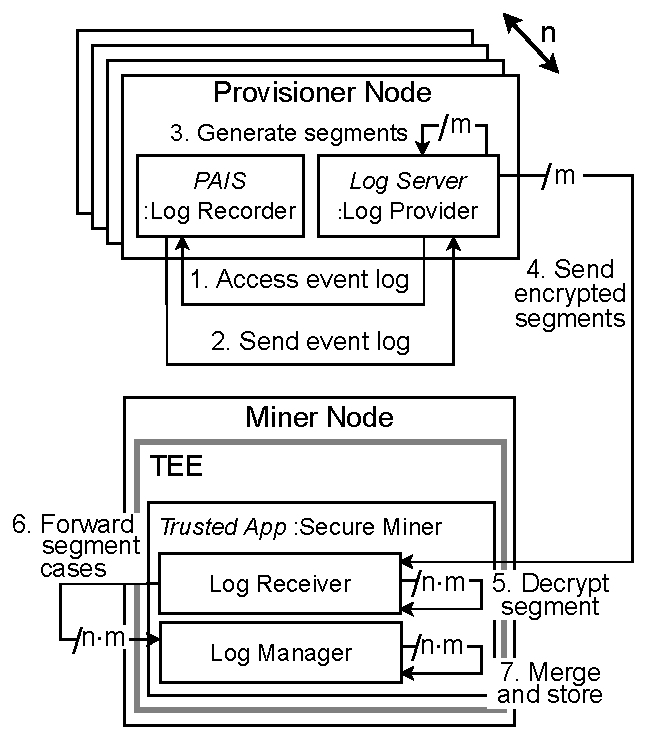
\includegraphics[width=0.4\linewidth]{content/figures/datatransmissionworkflow.pdf}\label{fig:transmission}}\hfill
	\subfloat[][Computation]{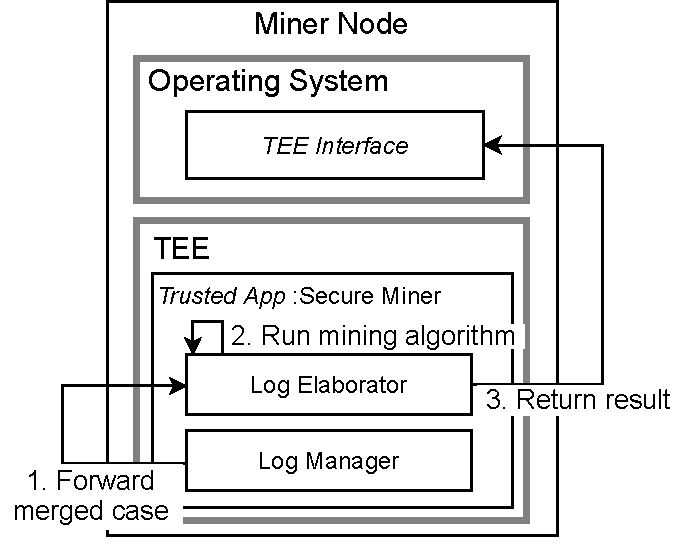
\includegraphics[width=0.45\linewidth]{content/figures/computationworkflow.pdf}\label{fig:computation}}\hfill	
	\caption{Unfolding example for the data transmission and computation phases of the CONFINE protocol}
	\label{fig:workflow}
\end{figure}
\noindent\textbf{Data transmission.} Once the trusted nature of the \Compo{Trusted App} is verified, the \Compo{Log Server}s proceed with the transmission of their cases. To accomplish this, each \Compo{Log Server} retrieves the event log from the \Compo{PAIS} (steps 1 and 2 in \cref{fig:transmission}), and filters it according to the case reference set specified by the miner. Given the constrained workload capacity of the \Compo{TEE}, it is imperative for \Compo{Log Server}s to partition the filtered event log into distinct segments. %We take this precautionary measure to avert runtime crashes. 
Consequently, each \Compo{Log Server} generates $m$ log segments comprising a variable count of entire cases (3 and \crefalgln[alg:lprv]{alg:lprv:logaccess}). The cumulative size of these segments is governed by the threshold parameter specified by the miner in the initial request (step 1 of the remote attestation phase, \cref{fig:attestation}). As an illustrative example from our motivating scenario, the \Compo{Log Server} of the \Actor{Hospital} may structure the segmentation such that $T^H_{312}$ and $T^H_{711}$ reside within the same segment, whereas the \Actor{Specialized clinic} might have $T^S_{312}$ and $T^S_{711}$ in separate segments. Subsequently, the $n$ \Compo{Log Server}s transmit their $m$ encrypted segments to the \Compo{Log Receiver} of the \Compo{Trusted App} (4 and \crefalgln[alg:lprv]{alg:lprv:sendSegs}). The \Compo{Log Receiver}, in turn, collects the $n \times m$ responses in a queue, processing them one at a time. After decrypting the processed segment (5), the \Compo{Log Receiver} forwards the cases contained in the segment to the \Compo{Log Manager} (6 and \crefalgln[alg:secm]{alg:secm:mergeAndStore}). To reconstruct the process instance, cases belonging to the same process instance must be merged by the \Compo{Log Manager} resulting in a single trace (e.g., $T_{312}$ for Alice case) comprehensive of all the events in the partial traces (e.g., $T^H_{312}$, $T^S_{312}$ and $T^C_{312}$ for Alice case). During this operation, the \Compo{Log Manager} applies a specific \textit{merging schema} (i.e., a rule specifying the attributes that link two cases during the merge) as stated in \citep{claes2014merging}. In our illustrative scenario, the merging schema to combine the cases of Alice is contingent upon the linkage established through their case identifier (i.e., 312). We underline that our proposed solution facilitates the incorporation of diverse merging schemas encompassing distinct trace attributes. The outcomes arising from merging the cases within the processed segment are securely stored by the \Compo{Log Manager} in the \Compo{TEE}.

\begin{comment}
\begin{wrapfigure}[8]{r}{0.4\textwidth}
%	\vspace{-1em}
	%\centering
	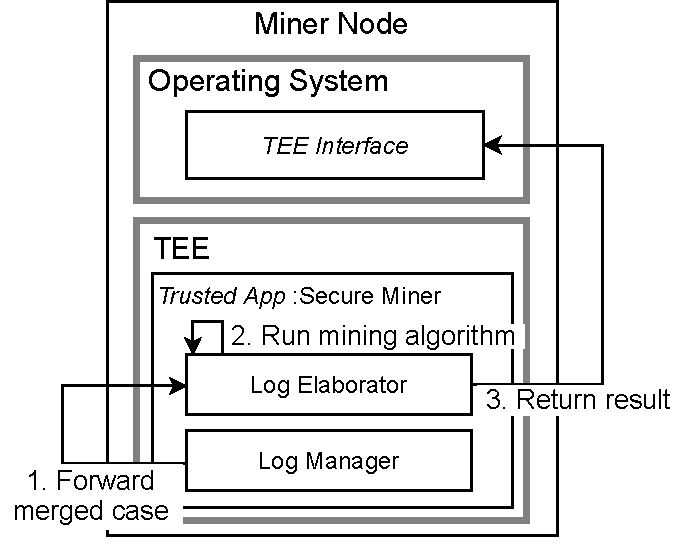
\includegraphics[width=\textwidth]{content/figures/computationworkflow.pdf}
	\caption[A gull]{Computation phase of the CONFINE protocol}
	\vspace{-2pt}
	\label{fig:computation}
\end{wrapfigure}
\end{comment}
\noindent\textbf{Computation.} The \texttt{Trusted App} requires all the provisioners to have delivered cases referring to the same process instances. For example, when the \Actor{Hospital} and the other organizations have all delivered their information concerning case 312 to the \Compo{Trusted App}, the process instance associated with Alice becomes eligible for computation. Upon meeting this condition (\crefalgln[alg:secm]{alg:secm:computation}), the \Compo{Log Manager} forwards the case earmarked for computation to the \Compo{Log Elaborator} (step 1 in \cref{fig:computation} and \crefalgln[alg:secm]{alg:secm:yield}). Subsequently, the \Compo{Log Elaborator} proceeds to input the merged case into the process mining algorithm (2). Ultimately, the outcome of the computation is relayed by the \Compo{Log Elaborator} from the \Compo{TEE} to the \Compo{TEE Interface} running atop the \Compo{Operating System} of the \Compo{Miner Node} (3). The CONFINE protocol does not impose restrictions on the post-computational handling of results. In our motivating scenario, the University and the National Institute of Statistics, serving as miners, disseminate the outcomes of computations, generating analyses that benefit the provisioners (though the original data are never revealed in clear). Furthermore, our protocol enables the potential for provisioners to have their proprietary \Compo{Secure Miner}, allowing them autonomous control over the computed results.

\subsection{Implementation}
\label{sec:implementation:details}
\begin{newj}
We implemented the \texttt{Secure Miner} component as an Intel SGX\footnote{\url{sgx101.gitbook.io/sgx101/}. Accessed: \today.} trusted application, encoded in Go through the EGo framework.\footnote{\url{docs.edgeless.systems/ego}. Accessed: \today.} With the same programming language we produced a the provisioner's \Compo{Log Server} implementation. 
The implementation of our \Compo{Secure Miner} component facilitates input reception from local users via a console application (\Compo{TEE Interface in \cref{sec:deployment}}). We store the descriptive information of the \Compo{Trusted App} (i,e., heap size, embedded files, and environment variables) in a JSON file. The EGo framework automatically generates an RSA key pair uniquely associated with the developer of the \Compo{Trusted App}. This key pair is stored in a PEM file. In our implementation, the \Compo{Secure Miner} app maintains references to provisioners' \Compo{Log Server}s in a dedicated JSON file, alongside the label of the {\CId} attribute in their respective log partitions. We assume this configuration file to be embedded in the \Compo{TEE} during deployment. We resort to a TLS~\citep{Thomas/2000:SSL-TLS} communication channel between miners and provisioners over the HTTP web protocol to secure the information exchange. To verify the trusted nature of the \Compo{Secure Miner}, we employ the SGX DCAP attestation scheme as the underlying backbone for our \emph{remote attestation} phase. The control data structures {\CIDMap} and {\LPrvMap} (refer to \cref{alg:secm}) generated by the \Compo{Secure Miner} during the CONFINE protocol are formatted as JSON files. To enable our miner \Compo{Trusted App} to handle provisioners' event logs, we implements an XES parser operating within the \Compo{Log Elaborator} of the \Compo{Secure Miner}. Upon successful execution, our \textit{HeuristicsMiner} implementation generates workflow nets corresponding to the analyzed processes.The \Compo{Secure Miner} presents the output process models computed by the \textit{HeuristicsMiner} in the PNML data format. 

Our implementation of CONFINE, including the \textit{HeuristicsMiner} in Go, is openly accessible at the following URL: \href{https://github.com/Process-in-Chains/CONFINE/}{\nolinkurl{github.com/Process-in-Chains/CONFINE/}}.    


%\todo[inline]{Add details on:
%enclave json\\
%public and private keys\\
%Communication protocol HTTP\\
%Metadata structures\\
%Authentication mechanism and security channel\\
%Remote attestation model\\
%Data transmission and integrity check\\
%Event log store\\
%Computation phase: Algorithms implemented\\
%Output: format and location of the results\\
%Datasets\\
%}
\end{newj}
%We resort to a TLS~\citep{Thomas/2000:SSL-TLS} communication channel between miners and provisioners over the HTTP web protocol to secure the information exchange. To demonstrate the effectiveness of our framework, we re-implemented and integrated the \textit{HeuristicsMiner} discovery algorithm~\citep{weijters2006process} within the \Compo{Trusted Application}. %Upon successful execution, our \textit{HeuristicsMiner} implementation generates workflow nets corresponding to the analyzed processes. Our implementation of CONFINE, including the \textit{HeuristicsMiner} in Go, is openly accessible at the following URL: \href{https://github.com/Process-in-Chains/CONFINE/}{\nolinkurl{github.com/Process-in-Chains/CONFINE/}}.
